%
% firmware.tex
%
% Copyright The TTC 2.0 Contributors.
%
% TTC 2.0 Documentation
%
% This work is licensed under the Creative Commons Attribution-ShareAlike 4.0
% International License. To view a copy of this license,
% visit http://creativecommons.org/licenses/by-sa/4.0/.
%

%
% \brief Firmware project chapter.
%
% \author Gabriel Mariano Marcelino <gabriel.mm8@gmail.com>
%
% \version 0.3.0
%
% \date 2021/05/12
%


\chapter{Firmware} \label{ch:firmware}

This chapter describes the main characteristics of the firmware part of the TTC module.

\section{Product tree}

The product tree of the firmware part of the TTC 2.0 module is available in \autoref{fig:product-tree-fw}. This product tree follows the architecture of the firmware, being divided according to the firmware layers.

\begin{figure}[!ht]
    \begin{center}
        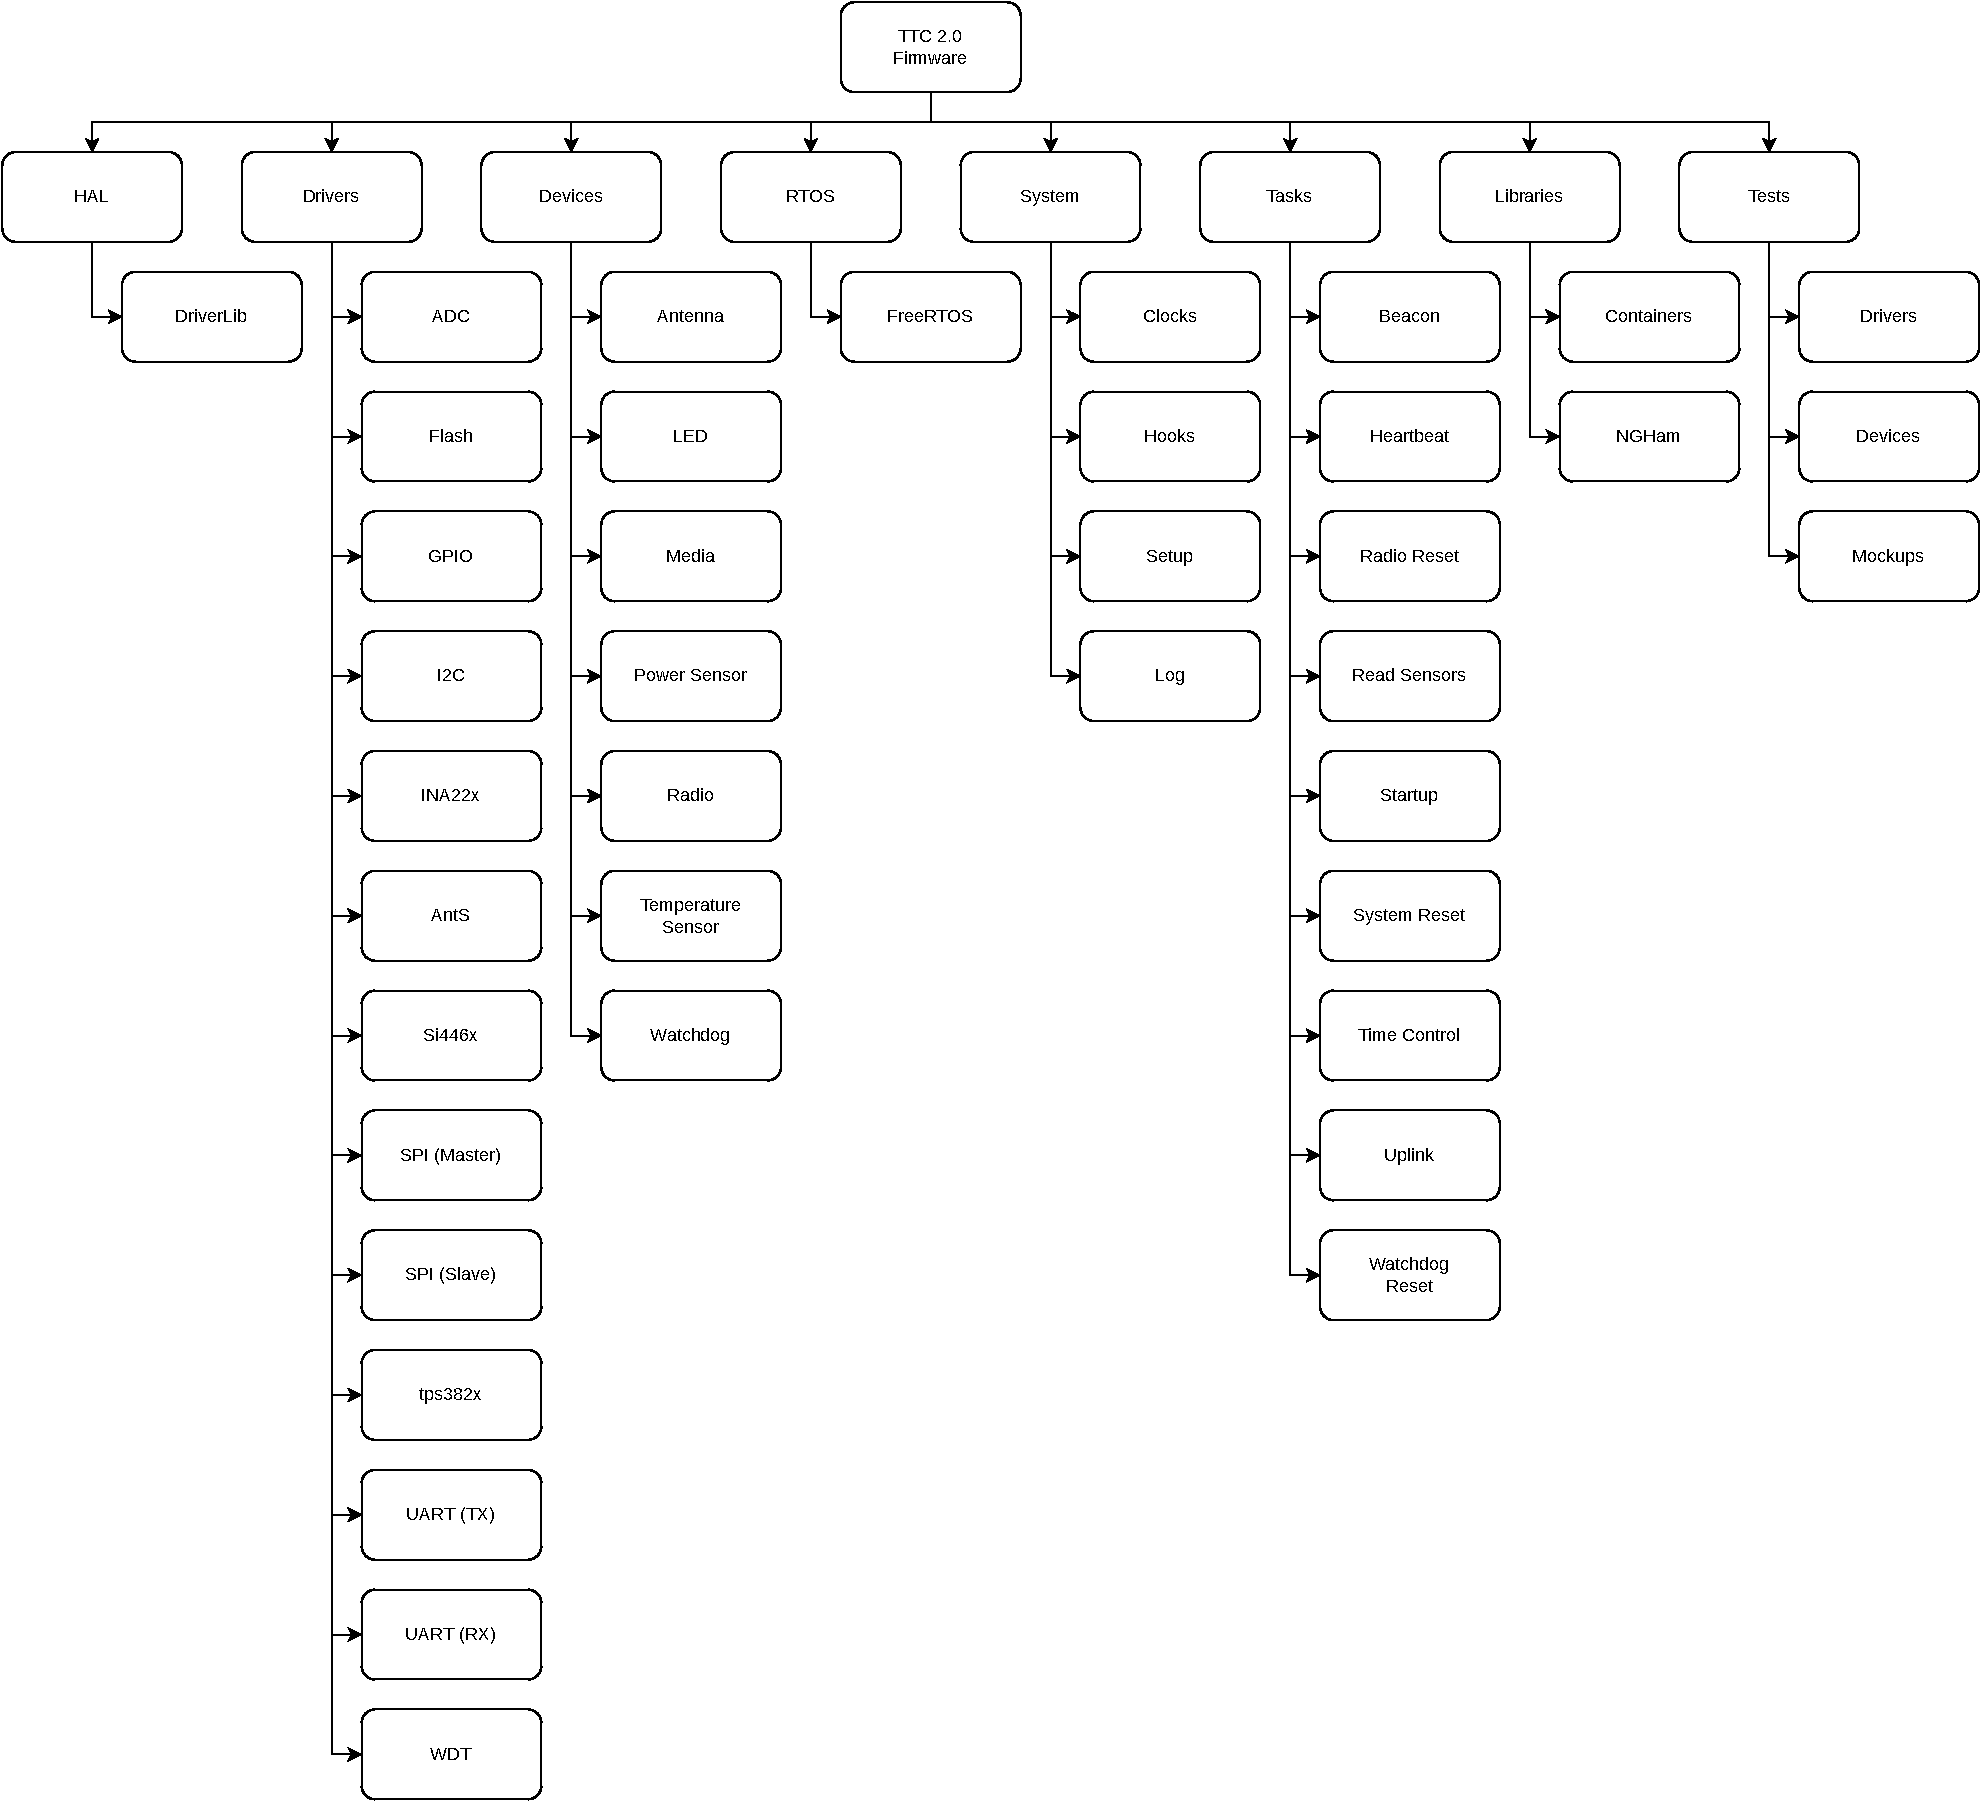
\includegraphics[width=\textwidth]{figures/product-tree-fw.pdf}
        \caption{Product tree of the firmware of the TTC 2.0 module.}
        \label{fig:product-tree-fw}
    \end{center}
\end{figure}

\section{Commands} \label{sec:commands}

To externally control and access the TTC module, some commands are available through the serial interfaces of the board. The commands are almost identical for both microcontrollers (except the command answering behavior) and are available on all interfaces. A list with the commands is available in \autoref{tab:commands}. The format of the commands' answers can be seen in \autoref{tab:commands-ans}.

\begin{table}[!ht]
    \centering
    \begin{tabular}{clll}
        \toprule[1.5pt]
        \textbf{ID} & \textbf{Name} & \textbf{Content} & \textbf{Interface}\\
        \midrule
        0   & NOP               & None                                           & SPI \\
        1   & Read parameter    & Parameter ID (1B) + Value (4B) + Checksum (2B) & SPI/UART \\
        2   & Write parameter   & Parameter ID (1B) + Value (4B) + Checksum (2B) & SPI/UART \\
        3   & Transmit packet   & Packet data (1-220B) + Checksum (2B)           & SPI/UART \\
        4   & Receive packet    & Packet data (1-220B) + Checksum (2B)           & SPI/UART \\
        \bottomrule[1.5pt]
    \end{tabular}
    \caption{List of commands.}
    \label{tab:commands}
\end{table}

\begin{table}[!ht]
    \centering
    \begin{tabular}{cll}
        \toprule[1.5pt]
        \textbf{ID} & \textbf{Name} & \textbf{Content}\\
        \midrule
        1   & Read parameter    & Parameter ID (1B) + Value (4B) + Checksum (2B) \\
        2   & Write parameter   & None \\
        3   & Transmit packet   & None \\
        4   & Receive packet    & Packet data (1-220B) + Checksum (2B) \\
        \bottomrule[1.5pt]
    \end{tabular}
    \caption{Format of the command's answers.}
    \label{tab:commands-ans}
\end{table}

All commands are composed of an ID field (1 byte), the content of the command, and a checksum at the end of the command (2 bytes). The used checksum algorithm is the CRC16-CCITT\nomenclature{\textbf{CRC}}{\textit{Cyclic Redundancy Check.}} \nomenclature{\textbf{CCITT}}{\textit{Comité Consultatif International Téléphonique et Télégraphique.}} (initial value = 0x0000, polynomial = 0x1021). The CRC value is calculated with the entire packet (ID field + command content).

A description of each command is available below:

\begin{itemize}
    \item NOP (No Operation, ID = 1): This command does nothing on the TTC; it is used for reading operations on the SPI interface when an answer to a telecommand is required.
    \item Read parameter/variable (ID = 1): This command is used to read a parameter or variable of the TTC module. It is composed of the command ID (1 byte), the parameter ID (1 byte), and the checksum value (2 bytes). After receiving the command, the answer with the parameter's value can be read with the NOP command (using the SPI interface, with the UART interface, the answer is immediately transmitted). The answer is composed of the command ID (1 byte), the parameter ID (1 byte), the parameter or variable value (4 bytes), and the checksum value (2 bytes).
    \item Write parameter/variable (ID = 2): This command is used to write a value to a given parameter or variable when allowed. It is composed of the command ID (1 byte), the parameter ID (1 byte), the new value of the parameter (4 bytes), and the checksum value (2 bytes). This command has no answer.
    \item Transmit packet (ID = 3): This command is used to transmit a packet through the radio link of each microcontroller. It is composed of the command ID (1 byte), the payload of the packet (1 to 220 bytes), and the checksum value (2 bytes). After receiving it, the TTC immediately transmits a new NGHam packet if the transmissions are enabled. This command has no answer.
    \item Receive packet (ID = 4): This command is used to read a received packet through the radio link (stored in the internal FIFO of the microcontrollers of the TTC). It comprises just the command ID (1 byte) and the checksum value (2 bytes). After receiving it, the TTC immediately allows access to the first available packet. The answer to this command, composed of the command ID (1 byte), the packet content (1 to 220 bytes), and the checksum value (2 bytes) can be read using the NOP command.
\end{itemize}

\section{Variables and Parameters} \label{sec:variables}

A list of all the variables of TTC with their identification number (ID) and variable type that can be read from the sensors and peripherals can be seen in \autoref{tab:ttc2-variables}.

\begin{longtable}[c]{cL{0.72\textwidth}lc}
    \toprule[1.5pt]
    \textbf{ID} & \textbf{Name/Description} & \textbf{Type} & \textbf{Access} \\
    \midrule
    0   & Device ID (0xCC2A or 0xCC2B)                                      & uint16 & R \\
    1   & Hardware version                                                  & uint8  & R \\
    2   & Firmware version (ex.: ``v1.2.3''' = 0x00010203)                  & uint32 & R \\
    3   & Time counter in milliseconds                                       & uint32 & R \\
    4   & Reset counter                                                     & uint16 & R \\
    \multirow{18}{*}{5} & Last reset cause: & \multirow{18}{*}{uint8} & \multirow{18}{*}{R} \\
        & - 0x00 = No interrupt pending                                     &        &  \\
        & - 0x02 = Brownout (BOR)                                           &        &  \\
        & - 0x04 = RST/NMI (BOR)                                            &        &  \\
        & - 0x06 = PMMSWBOR (BOR)                                           &        &  \\
        & - 0x08 = Wakeup from LPMx.5 (BOR)                                 &        &  \\
        & - 0x0A = Security violation (BOR)                                 &        &  \\
        & - 0x0C = SVSL (POR)                                               &        &  \\
        & - 0x0E = SVSH (POR)                                               &        &  \\
        & - 0x10 = SVML\_OVP (POR)                                          &        &  \\
        & - 0x12 = SVMH\_OVP (POR)                                          &        &  \\
        & - 0x14 = PMMSWPOR (POR)                                           &        &  \\
        & - 0x16 = WDT time out (PUC)                                       &        &  \\
        & - 0x18 = WDT password violation (PUC)                             &        &  \\
        & - 0x1A = Flash password violation (PUC)                           &        &  \\
        & - 0x1C = Reserved                                                 &        &  \\
        & - 0x1E = PERF peripheral/configuration area fetch (PUC)           &        &  \\
        & - 0x20 = PMM password violation (PUC)                             &        &  \\
        & - 0x22 to 0x3E = Reserved                                         &        &  \\
    6   & Input voltage of the $\mu$C in mV                                 & uint16 & R \\
    7   & Input current of the $\mu$C in mA                                 & uint16 & R \\
    8   & Temperature of the $\mu$C in K                                    & uint16 & R \\
    9   & Input voltage of the radio in mV                                  & uint16 & R \\
    10  & Input current of the radio in mA                                  & uint16 & R \\
    11  & Temperature of the radio in K                                     & uint16 & R \\
    12  & Last valid command (uplink packet ID)                             & uint8  & R \\
    13  & RSSI of the last valid telecommand                                & uint16 & R \\
    14  & Temperature of the antenna module in K                            & uint16 & R \\
    \multirow{17}{*}{15} & Antenna module status bits:                      & \multirow{17}{*}{uint16} & \multirow{17}{*}{R} \\
        & - Bit 15: The antenna 1 is deployed (0) or not (1)                &        &   \\
        & - Bit 14: Cause of the latest activation stop for antenna 1       &        &   \\
        & - Bit 13: The antenna 1 deployment is active (1) or not (0)       &        &   \\
        & - Bit 11: The antenna 2 is deployed (0) or not (1)                &        &   \\
        & - Bit 10: Cause of the latest activation stop for antenna 2       &        &   \\
        & - Bit 9: The antenna 2 deployment is active (1) or not (0)        &        &   \\
        & - Bit 8: The antenna is ignoring the deployment switches (1) or not (0) &  &   \\
        & - Bit 7: The antenna 3 is deployed (0) or not (1)                 &        &   \\
        & - Bit 6: Cause of the latest activation stop for antenna 3        &        &   \\
        & - Bit 5: The antenna 3 deployment is active (1) or not (0)        &        &   \\
        & - Bit 4: The antenna system independent burn is active (1) or not (0) &    &   \\
        & - Bit 3: The antenna 4 is deployed (0) or not (1)                 &        &   \\
        & - Bit 2: Cause of the latest activation stop for antenna 4        &        &   \\
        & - Bit 1: The antenna 4 deployment is active (1) or not (0)        &        &   \\
        & - Bit 0: The antenna system is armed (1) or not (0)               &        &   \\
    16  & Antenna deployment status (0=never executed, 1=executed)          & uint8  & R \\
    17  & Antenna deployment hibernation (0=never executed, 1=executed)     & uint8  & R \\
    18  & TX enable (0=off, 1=on)                                           & uint8  & R/W \\
    19  & TX packet counter                                                 & uint32 & R \\
    20  & RX packet counter (valid packets)                                 & uint32 & R \\
    21  & TX packets available in the FIFO buffer                           & uint8  & R \\
    22  & RX packets available in the FIFO buffer                           & uint8  & R \\
    23  & Number of bytes of the first available packet in the RX buffer    & uint16 & R \\
    \bottomrule[1.5pt]
    \caption{Variables and parameters of the TTC 2.0.}
    \label{tab:ttc2-variables}
\end{longtable}

Each variable can be read or written using the commands ``Read Parameter'' and/or ``Write Parameter''. Some variables can just be read, as seen in the most right column of \autoref{tab:ttc2-variables}. When a variable is less than 32 bits long, it is left filled with zeros during a read or write operation (ex.: the value 0xAB becomes 0x000000AB).

\section{Layers}

The firmware flow of development goes from the low-level implementation (far right), with HA layer being register-level operation, to Tasks Layer with very abstract and high-level code.

\subsection{Hardware Abstraction Layer (HAL)}

The HAL layer is the API DriverLib developed by Texas Instruments; it includes register manipulating functions to accelerate development. The TTC 2.0 uses HAL to handle GPIO operations and serial communications such as SPI, UART, and I$^2$C.

\subsection{Drivers}

Driver Layer is created to have the flexibility of the HAL layer but contains only the necessary abstraction to be still generic enough to support all the functionalities needed in Devices or other Drivers modules.

\subsection{Devices}

In this level of abstraction, the devices are used to create specific configurations with the Drivers Layer to build functions used in the Tasks layer. In opposition to the Drivers layer, the Devices do not communicate between themselves and are only used inside Tasks.

\subsection{RTOS}

The TTC 2.0 uses FreeRTOS kernel. Using an RTOS-based kernel enables the system to regularly maintain routine functions such as housekeeping, sensor reading, checking for receptions, and dealing with specific delays used in hardware, such as the radio. The priority level of a task dictates who has the most preference for execution. Initial delay and period are used to determine the delay time to execute the task initialization after a boot; this regulates the time between the task executions. The stack is the amount of memory delimited to execute a task.

\subsection{System}

The System layer is used for housekeeping and management routines; it contains the system log, clock setup, and hooks. Its executions occur in almost all the TTC 2.0 abstraction layers (except the Tests layer), mostly for log purposes, as seen in Figure \ref{fig:log_info}.

\begin{figure}[!ht]
	\begin{center}
		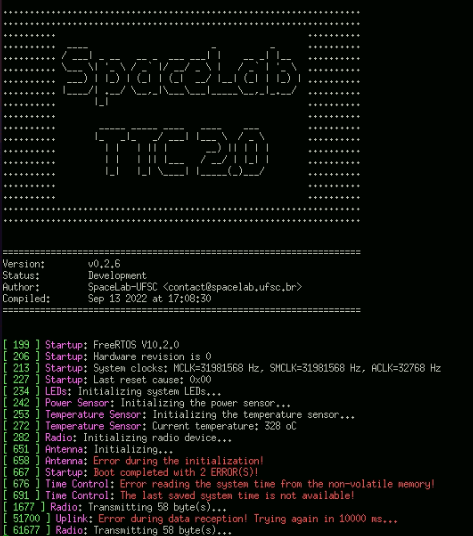
\includegraphics[width=0.65\textwidth]{figures/ttc2-terminal-log.png}
		\caption{Example of log feedback received from TTC 2.0 during debug.}
		\label{fig:log_info}
	\end{center}
\end{figure}

\subsection{Tasks}

Tasks are the FreeRTOS threads equivalent and are the uppermost abstraction layer of code inside the TTC 2.0 flow of execution. Each task is designated a priority level, initial delay, period, and stack size as shown in \autoref{tab:firmware-tasks}.

\begin{table}[!ht]
    \centering

    \begin{tabular}{lccccc}
        \toprule[1.5pt]
        \textbf{Name}          & \textbf{Priority} & \textbf{Initial delay [ms]} & \textbf{Period [ms]} & \textbf{Stack [bytes]} \\
        \midrule
        Automatic Beacon       & High    & 60000 & 60000     & 300 \\
        Command Processing     & Highest & 0     & 100       & 500 \\
        Heartbeat              & Lowest  & 0     & 500       & 160 \\
        Housekeeping           & Medium  & 2000  & 10000     & 160 \\
        Radio Reset            & High    & 60000 & 60000     & 128 \\
        Startup                & Medium  & 0     & Aperiodic & 128 \\
        System Reset           & Medium  & 0     & 36000000  & 128 \\
        Time Control           & Medium  & 1000  & 1000      & 128 \\
        Uplink                 & Highest & 2000  & 500       & 500 \\
        Watchdog Reset         & Lowest  & 0     & 100       & 150 \\
        \bottomrule[1.5pt]
    \end{tabular}
    \caption{List of TTC 2.0 Tasks with configuration parameters.}
    \label{tab:firmware-tasks}
\end{table}

Each of the tasks presented in \autoref{tab:firmware-tasks} is described below:

\begin{itemize}
    \item \textbf{Automatic Beacon}: Automatically transmits a beacon packet if no transmission command is received within 60 seconds.
    \item \textbf{Command Processing}: Process incoming commands (physical interfaces).
    \item \textbf{Heartbeat}: Blinks a status LED at a rate of 1 Hz. Both microcontrollers have a status LED. This LED indicates that the scheduler is up and running.
    \item \textbf{Housekeeping}: This task manages the general operation of the TTC.
    \item \textbf{Radio Reset}: Resets the radio at 600 seconds.
    \item \textbf{Startup}: Initializes all the devices and peripherals, and variables of the TTC 2.0 module (boot sequence).
    \item \textbf{System Reset}: Resets the microcontroller by software every 10 hours.
    \item \textbf{Time Control}: Manages the system time by loading the saving the time counter from/to the FRAM memory.
    \item \textbf{Uplink}: Monitors the radio module for upcoming packages and stores it in memory.
    \item \textbf{Watchdog Reset}: Resets both watchdog timers (internal and external) at every 100 milliseconds.
\end{itemize}

\subsection{Libraries}

The Libraries are used for algorithm purposes and are not related to any hardware. Their function removes the redundancy of creating multiple identical structures for different driver modules.

\subsection{Tests}

Tests are used to verify and validate the Drivers and Devices' developed functionality. There are three types of tests: the static test uses the MISRA C: 2012 \cite{misrac2012} guidelines to check for C safety standards, the unitary tests use the Cmocka\footnote{\href{https://cmocka.org/}{https://cmocka.org/}} library with mockups of the hardware, to validate the module in an algorithmic level, and the last test verifies the integration between hardware and firmware.
